\documentclass[12pt,letterpaper]{article}
\usepackage[utf8]{inputenc}
\usepackage[letterpaper, margin=1in, bottom=2.5in, top=1.2in]{geometry}
\usepackage{fancyhdr}
\setlength{\headheight}{15pt}
\setlength{\footskip}{72pt}

\usepackage{xcolor}
\usepackage{amsmath}
\usepackage{anyfontsize}
\usepackage{graphicx}
\usepackage{tikz}
\usepackage{listings}
\usepackage{sourcesanspro}
\renewcommand{\familydefault}{\sfdefault}
\usepackage{fontawesome5}
\usepackage{titlesec}
\usepackage{setspace}
\usepackage{hyperref}
\usepackage{mdframed}
\usepackage{qrcode} % Added QR code package
\usetikzlibrary{calc,shapes,positioning}

\AtBeginDocument{\color{primaryColor}}

% Colors
\definecolor{bgColor}{RGB}{16, 24, 47}
\definecolor{primaryColor}{RGB}{255, 255, 255}
\definecolor{accentColor}{RGB}{142, 152, 255}
\definecolor{pythonBlue}{RGB}{142, 152, 255}
\definecolor{secondaryColor}{RGB}{200, 200, 200}
\definecolor{terminalBg}{RGB}{20, 28, 50}
\definecolor{terminalFrame}{RGB}{45, 53, 80}
\definecolor{lineNumberColor}{RGB}{120, 160, 200}
\definecolor{dividerColor}{RGB}{45, 53, 80}

% Code colors
\definecolor{codeTextColor}{RGB}{255, 255, 255}
\definecolor{codeKeywordColor}{RGB}{215, 130, 240}
\definecolor{codeCommentColor}{RGB}{120, 160, 200}
\definecolor{codeStringColor}{RGB}{170, 220, 130}
\definecolor{codeMethodColor}{RGB}{142, 152, 255}
\definecolor{codeFunctionColor}{RGB}{170, 220, 130}
\definecolor{codeNumberColor}{RGB}{255, 255, 150}

\pagecolor{bgColor}

\hypersetup{
    colorlinks=true,
    linkcolor=accentColor,
    filecolor=accentColor,
    urlcolor=accentColor,
}

\lstset{
  language=Python,
  basicstyle=\small\ttfamily\bfseries\color{codeTextColor},
  backgroundcolor=\color{terminalBg},
  commentstyle=\color{codeCommentColor},
  keywordstyle=\color{codeKeywordColor},
  stringstyle=\color{codeStringColor},
  numberstyle=\color{lineNumberColor},
  breaklines=true,
  breakatwhitespace=true,
  tabsize=4,
  showstringspaces=false,
  frame=none,
  xleftmargin=15pt,
  xrightmargin=0pt,
  aboveskip=5pt,
  belowskip=5pt,
  numbers=left,
  numbersep=8pt,
  extendedchars=true,
  keepspaces=true,
  columns=flexible,
  lineskip=2pt,
  morekeywords={self, yield, lambda, with, as, from, True, False, None, import, in, for, 
                if, elif, else, while, return, def, class, try, except, finally, raise, 
                break, continue, global, nonlocal, pass, assert, del},
  emph={[2]print,range,sum,int,str,float,list,dict,set,tuple,next,len,type,map,filter,
         reduce,zip,enumerate,sorted,reversed,min,max,open,any,all},
  emphstyle={[2]\color{codeFunctionColor}}
}

\newenvironment{macterminal}{%
    \begin{mdframed}[
        linecolor=terminalFrame,
        backgroundcolor=terminalBg,
        roundcorner=5pt,
        skipabove=5pt,
        skipbelow=5pt,
        linewidth=1pt,
        innertopmargin=5pt,
        frametitle={%
            \tikz[baseline=(current bounding box.east), outer sep=0pt]{
                \fill[red!80!black] (0,0) circle (5pt);
                \fill[yellow!80!black] (0.7,0) circle (5pt);
                \fill[green!70!black] (1.4,0) circle (5pt);
            }
        },
        frametitlealignment=\raggedright,
        frametitleaboveskip=8pt,
        frametitlebelowskip=0pt,
    ]
}{%
    \end{mdframed}%
}

% Added elegantqr command
\newcommand{\elegantqr}[2]{
    \qrcode[height=2.5cm]{#1}
    \\[0.1cm]
    {\hspace{0.2cm}\color{primaryColor}\small #2\par}
}

\newcommand{\verspace}{\vspace{5pt}}

\titleformat{\section}
  {\LARGE\bfseries\color{accentColor}}
  {\thesection. }
  {0pt}
  {}
  []

\titleformat{\subsection}
  {\Large\bfseries\color{pythonBlue}}
  {\thesubsection. }
  {0pt}
  {}
  []

\titleformat{\subsubsection}
  {\large\bfseries\color{accentColor}}
  {\thesubsubsection. }
  {0pt}
  {}
  []

\titlespacing*{\section}{0pt}{18pt}{8pt}
\titlespacing*{\subsection}{0pt}{12pt}{5pt}
\titlespacing*{\subsubsection}{0pt}{8pt}{3pt}

\pagestyle{fancy}
\fancyhf{}

\fancyhead[L]{
    
\begin{tikzpicture}[remember picture, overlay]
        \fill[pythonBlue, rounded corners=3pt] (0,0) rectangle (2.2cm,0.7cm);
        \node[text=primaryColor, font=\bfseries] at (1.1cm,0.35cm) {AI};
        \fill[secondaryColor] (2.35cm,0.1cm) rectangle (2.40cm,0.6cm);
        \node[text=accentColor, font=\bfseries, anchor=west] at (2.35cm,0.35cm) {REASONING FRAMEWORKS};
    \end{tikzpicture}
}

\renewcommand{\headrulewidth}{0pt}

\renewcommand{\footrule}{
  \vspace{0.5cm}
  \noindent\makebox[\linewidth]{\color{dividerColor}\rule{\linewidth}{0.2pt}}
  \vspace{0.5cm}
}
\renewcommand{\footrulewidth}{0.2pt}
\renewcommand{\footruleskip}{1cm}

\fancyfoot[C]{
    \vspace*{0.1cm}
    \noindent
    \begin{minipage}{\textwidth}
        \begin{flushleft}
            \raisebox{0.7cm}{
            \begin{tikzpicture}[baseline]
                \path[fill=bgColor] (0,0) circle (0.6cm);
                \clip (0,0) circle (0.6cm);
                \node at (0,0) {
                    
\includegraphics[width=1.2cm,height=1.2cm]{profile-image.jpeg}
                };
            \end{tikzpicture}
            }
            \begin{minipage}[b]{0.8\textwidth}
                {\large\bfseries\color{primaryColor}Alejandro Sánchez Yalí}
                \par\vspace{1pt}
                {\small\color{secondaryColor}Software Developer | AI \& Blockchain Enthusiast}
                \par\vspace{1pt}
                {\small\color{accentColor}\faGlobe\hspace{5pt}\color{secondaryColor}www.asanchezyali.com}
            \end{minipage}
        \end{flushleft}
        \vspace{6pt}
    \end{minipage}
}

\fancypagestyle{plain}{
    \fancyhf{}
    \renewcommand{\headrulewidth}{0pt}
    \renewcommand{\footrulewidth}{0pt}
}

\renewcommand{\labelitemi}{\textcolor{accentColor}{$\bullet$}}
\renewcommand{\labelitemii}{\textcolor{pythonBlue}{$\circ$}}

\usepackage{relsize}
\AtBeginDocument{\relsize{1}}

\newcommand{\languagetag}[1]{
    \begin{tikzpicture}[baseline]
        \node[fill=pythonBlue, text=primaryColor, rounded corners=5pt, inner sep=7pt] {
            {\normalsize\textbf{#1}}
        };
    \end{tikzpicture}
}

\newcommand{\titlepagecontents}{%
    \vspace*{3cm}
    % Formatted similar to the Python generators document
    \begin{flushleft}
    \noindent\languagetag{Artificial Intelligence}\\[0.4cm]
    \noindent{\fontsize{48}{52}\bfseries\color{primaryColor}Reasoning \color{accentColor}Frameworks\par}
    \vspace{0.3cm}
    \noindent{\fontsize{18}{52}\color{secondaryColor}Effective Strategies for AI Problem-Solving\par}
    \vspace{0.3cm}
    \noindent{\color{secondaryColor}\today\par}
    \vspace{2cm}
    % Added QR code
    \elegantqr{https://github.com/asanchezyali/social-media-posts/tree/main/ArtificialIntelligence/ReasoningFrameworks}{Source Code}
    \end{flushleft}
}

\newcommand{\finalpagecontents}{%
    \vspace*{6cm}
    \begin{center}
        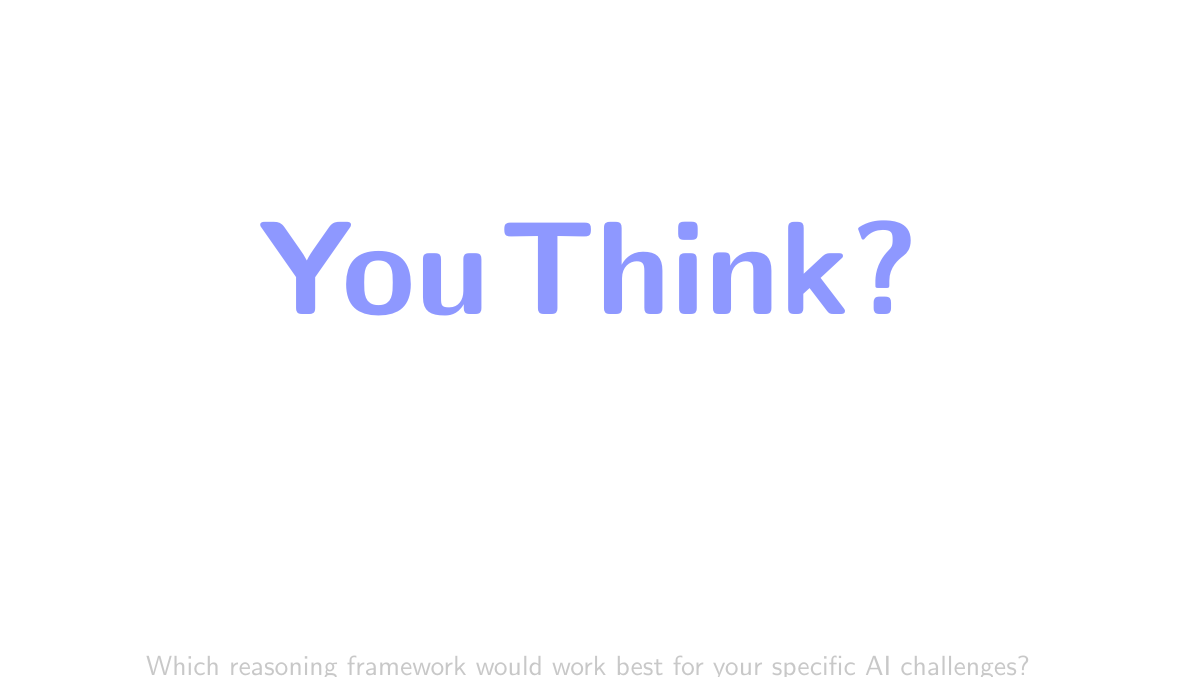
\begin{tikzpicture}
            % Title text
            \node[text width=14cm, align=center] at (0,0) {
                {\fontsize{48}{52}\bfseries\color{primaryColor}What Do \color{accentColor}You Think?\par}
            };
            
            % Add vertical space
            \node at (0,-3) {};
            
            % Question text
            \node[text width=14cm, align=center] at (0,-6) {
                {\fontsize{22}{26}\color{secondaryColor}Which reasoning framework would work best for your specific AI challenges?\par}
            };
        \end{tikzpicture}
    \end{center}
}

\begin{document}
\color{primaryColor}

\begin{titlepage}
    \titlepagecontents
\end{titlepage}

\section{Chain-of-Thought (CoT)}

Chain-of-Thought guides AI models to solve problems step-by-step, making their reasoning explicit.

\subsection{Key Points}
\begin{itemize}
    \item \textbf{\textcolor{pythonBlue}{What:}} Sequential reasoning that explicitly breaks down problem-solving into discrete, intermediate steps. The model articulates each stage of its thinking process, similar to how humans solve problems by making subgoals explicit.
    
    \item \textbf{\textcolor{pythonBlue}{Origin:}} Introduced by Wei et al. (2022) at Google Research. The technique emerged from observing that large language models perform better on complex tasks when prompted to generate explanatory steps before producing a final answer.
    
    \item \textbf{\textcolor{pythonBlue}{Strengths:}} Enhanced transparency allows users to inspect the reasoning process; significantly improved performance on mathematical reasoning (40-80\% accuracy gains in some tasks); enables better debugging of AI thinking; makes errors in logic more visible and correctable.
    
    \item \textbf{\textcolor{pythonBlue}{Weaknesses:}} Limited to examining only one solution path; errors early in the chain compound and propagate; not well-suited for problems requiring creative exploration or hypothesis testing; the linear nature prevents backtracking when reaching dead ends.
\end{itemize}

\subsection{Implementation Example}

\begin{macterminal}
\begin{lstlisting}
from langchain.prompts import PromptTemplate
from langchain.chains import LLMChain
from langchain.llms import OpenAI

# Optimized CoT prompt 
cot_prompt = PromptTemplate(
    input_variables=["question"],
    template="""
    Question: {question}
    To solve this, I will break it down into steps:
    1. Identify key components of the question.
    2. Apply reasoning to each component.
    3. Combine results for final answer.
    """
)

# Lower temperature for precision in calculations
llm = OpenAI(temperature=0.3)
chain = LLMChain(llm=llm, prompt=cot_prompt)

# Example: "If a shirt costs $20 after a 20% discount, what was its original price?"
\end{lstlisting}
\end{macterminal}

\section{Tree-of-Thoughts (ToT)}

Tree-of-Thoughts explores multiple reasoning paths simultaneously to find optimal solutions.

\subsection{Key Points}
\begin{itemize}
    \item \textbf{\textcolor{pythonBlue}{What:}} A hierarchical reasoning system that creates and evaluates multiple thought branches simultaneously. The model explores different solution strategies, evaluates their potential, and selectively explores the most promising paths—analogous to a chess player considering several moves ahead.
    
    \item \textbf{\textcolor{pythonBlue}{Origin:}} Developed by Yao et al. (2023) at Princeton University as an evolution of Chain-of-Thought. It was designed to overcome the limitations of linear reasoning in more complex or ambiguous problem spaces.
    
    \item \textbf{\textcolor{pythonBlue}{Strengths:}} Significantly more effective for complex planning problems and creative tasks; enables consideration of alternative hypotheses; allows backtracking when a path proves unfruitful; provides self-evaluation capabilities where the model itself can judge the quality of different approaches.
    
    \item \textbf{\textcolor{pythonBlue}{Weaknesses:}} Substantially more resource-intensive due to tracking multiple paths; implementation complexity increases with branch depth; can become unwieldy for human interpretation as the tree grows; requires careful design of evaluation strategies for pruning suboptimal branches.
\end{itemize}

\subsection{Implementation Example}

\begin{macterminal}
\begin{lstlisting}
from langchain.chains import LLMChain
from langchain.prompts import PromptTemplate
from langchain.llms import OpenAI

# ToT prompt with multiple solution paths
tot_prompt = PromptTemplate(
    input_variables=["question"],
    template="""
    Question: {question}
    Let's explore multiple approaches:
    1. Approach 1: [First potential solution]
    2. Approach 2: [Alternative solution]
    3. Evaluation: [Compare approaches]
    """
)

# Higher temperature for creative exploration
llm = OpenAI(temperature=0.7)
chain = LLMChain(llm=llm, prompt=tot_prompt)

# Example: "What's the best way to reduce energy consumption in a home?"
\end{lstlisting}
\end{macterminal}

\section{ReAct (Reasoning and Acting)}

ReAct integrates reasoning with real-time actions to access information and improve decisions.

\subsection{Key Points}
\begin{itemize}
    \item \textbf{\textcolor{pythonBlue}{What:}} A hybrid framework that interleaves reasoning steps with real-world actions. The model alternates between thinking internally and taking actions to gather information, creating a dynamic feedback loop between reasoning and environment interaction.
    
    \item \textbf{\textcolor{pythonBlue}{Origin:}} Introduced by Yao et al. (2022) at Princeton University and Google Research. The approach was inspired by how humans naturally combine reasoning with information-seeking actions when solving problems with incomplete information.
    
    \item \textbf{\textcolor{pythonBlue}{Strengths:}} Dramatically improves factual accuracy by grounding reasoning in real-time data; reduces hallucinations common in pure reasoning approaches; adapts dynamically to new information discovered during problem-solving; enables AI systems to leverage external tools, APIs, and knowledge bases.
    
    \item \textbf{\textcolor{pythonBlue}{Weaknesses:}} Significantly more complex to implement and orchestrate than pure reasoning frameworks; performance is heavily dependent on the quality and range of available tools; requires robust error handling for failed external actions; increased latency due to waiting for external systems.
\end{itemize}

\subsection{Implementation Example}

\begin{macterminal}
\begin{lstlisting}
from langchain.agents import initialize_agent, Tool
from langchain.llms import OpenAI

# Simulated search tool
def search_web(query):
    # This would connect to a real API in production
    if "capital of France" in query.lower():
        return "The capital of France is Paris."
    return "No specific information found."

search_tool = Tool(
    name="WebSearch",
    func=search_web,
    description="Searches for up-to-date information."
)

# Initialize ReAct agent with the tool
llm = OpenAI(temperature=0.5)
agent = initialize_agent(
    tools=[search_tool],
    llm=llm,
    agent_type="react",
    verbose=True
)

# Example: "What is the capital of France, and its population?"
\end{lstlisting}
\end{macterminal}

\section{Comparative Analysis}

\begin{center}
\begin{tabular}{|p{3cm}|p{4cm}|p{4cm}|p{4cm}|}
\hline
\small{\textbf{\textcolor{accentColor}{Aspect}}} & \small{\textbf{\textcolor{accentColor}{Chain-of-Thought}}} & \small{\textbf{\textcolor{accentColor}{Tree-of-Thoughts}}} & \small{\textbf{\textcolor{accentColor}{ReAct}}} \\
\hline
\small{\textbf{\textcolor{pythonBlue}{Best For}}} & 
\small{Math problems, sequential reasoning, step-by-step logic} & 
\small{Creative tasks, complex planning, multiple solution paths} & 
\small{Fact verification, research tasks, tool-dependent problems} \\
\hline
\small{\textbf{\textcolor{pythonBlue}{Compute}}} & 
\small{Low} & 
\small{High} & 
\small{Medium} \\
\hline
\small{\textbf{\textcolor{pythonBlue}{Implementation}}} & 
\small{Simple} & 
\small{Complex} & 
\small{Moderate} \\
\hline
\small{\textbf{\textcolor{pythonBlue}{Temperature}}} & 
\small{0.2-0.4} & 
\small{0.6-0.8} & 
\small{0.4-0.6} \\
\hline
\small{\textbf{\textcolor{pythonBlue}{Example Task}}} & 
\small{Solving equations, logical deduction} & 
\small{Essay writing, strategy games} & 
\small{Data analysis, answering factual questions} \\
\hline
\end{tabular}
\end{center}

\section{Emerging Hybrid Approaches}

\begin{itemize}
    \item \textbf{\textcolor{pythonBlue}{ReAct + ToT:}} Combines multiple reasoning paths with external actions for complex problems requiring information gathering and exploration
    
    \item \textbf{\textcolor{pythonBlue}{Reflexion:}} Extends ReAct with reinforcement learning (Shinn et al., 2023) to improve from past reasoning
    
    \item \textbf{\textcolor{pythonBlue}{Active Prompting:}} Enhances CoT by incorporating active learning principles (Diao et al., 2023)
    
    \item \textbf{\textcolor{pythonBlue}{Toolformer:}} Self-identifies when to use external tools during reasoning (Schick et al., 2023)
\end{itemize}

\section{Quick Implementation Tips}

\begin{itemize}
    \item \textbf{\textcolor{pythonBlue}{Choose Based On:}} Task structure, information needs, computational resources
    
    \item \textbf{\textcolor{pythonBlue}{Prompt Design:}} Explicitly guide the model's reasoning process matching the framework
    
    \item \textbf{\textcolor{pythonBlue}{Temperature:}} Adjust based on framework need (CoT: lower, ToT: higher)
    
    \item \textbf{\textcolor{pythonBlue}{Evaluation:}} Look beyond final answers to assess reasoning quality
\end{itemize}

\section{References}

\begin{itemize}
    \item Wei, J., et al. (2022). \textit{Chain-of-Thought Prompting Elicits Reasoning in Large Language Models}. arXiv:2201.11903. \href{https://arxiv.org/abs/2201.11903}{Link}
    \item Yao, S., et al. (2023). \textit{Tree of Thoughts: Deliberate Problem Solving with Large Language Models}. arXiv:2305.10601. \href{https://arxiv.org/abs/2305.10601}{Link}
    \item Yao, S., et al. (2022). \textit{ReAct: Synergizing Reasoning and Acting in Language Models}. arXiv:2210.03629. \href{https://arxiv.org/abs/2210.03629}{Link}
    \item Schick, T., et al. (2023). \textit{Toolformer: Language Models Can Teach Themselves to Use Tools}. \href{https://arxiv.org/abs/2302.04761}{Link}
    \item Diao, S., et al. (2023). \textit{Active Prompting with Chain-of-Thought for Large Language Models}. \href{https://arxiv.org/abs/2302.00923}{Link}
    \item Translated, Edited and written in collaboration with AI.
\end{itemize}

\clearpage
\thispagestyle{empty}
\finalpagecontents

\end{document}